% This is an example of using latex for a paper/report of specified
% size/layout. It's useful if you want to provide a PDF that looks
% like it was made in a normal word processor.

% While writing, don't stop for errors
\nonstopmode

% Use the article doc class, with an 11 pt basic font size
\documentclass[11pt, a4paper]{article}

% Makes the main font Nimbus Roman, a Times New Roman lookalike:
%\usepackage{mathptmx}% http://ctan.org/pkg/mathptmx
% OR use this for proper Times New Roman (from msttcorefonts package
% on Ubuntu). Use xelatex instead of pdflatex to compile:
\usepackage{fontspec}
\usepackage{xltxtra}
\usepackage{xunicode}
\defaultfontfeatures{Scale=MatchLowercase,Mapping=tex-text}
\setmainfont{Times New Roman}

% Nice citations
\usepackage{natbib}

% Set margins
\usepackage[margin=2.5cm]{geometry}

% Multilingual support
\usepackage[english]{babel}

% Nice mathematics
\usepackage{amsmath}

% Left right harpoons for kinetic equations
\usepackage{mathtools}

% Control over maketitle
\usepackage{titling}

% Section styling
\usepackage{titlesec}

% Ability to use colour in text
\usepackage[usenames]{color}

% For the \degree symbol
\usepackage{gensymb}

% Allow includegraphics and nice wrapped figures
\usepackage{graphicx}
\usepackage{wrapfig}
\usepackage[outercaption]{sidecap}

% Nice quotes
\usepackage{csquotes}

% Set formats using titlesec
\titleformat*{\section}{\bfseries\rmfamily}
\titleformat*{\subsection}{\bfseries\itshape\rmfamily}

% thetitle is the number of the section. This sets the distance from
% the number to the section text.
\titlelabel{\thetitle.\hskip0.3em\relax}

% Set title spacing with titlesec, too.  The first {1.0ex plus .2ex
% minus .7ex} sets the spacing above the section title. The second
% {-1.0ex plus 0.2ex} sets the spacing the section title to the
% paragraph.
\titlespacing{\section}{0pc}{1.0ex plus .2ex minus .7ex}{-1.1ex plus 0.2ex}

%% Trick to define a language alias and permit language = {en} in the .bib file.
% From: http://tex.stackexchange.com/questions/199254/babel-define-language-synonym
\usepackage{letltxmacro}
\LetLtxMacro{\ORIGselectlanguage}{\selectlanguage}
\makeatletter
\DeclareRobustCommand{\selectlanguage}[1]{%
  \@ifundefined{alias@\string#1}
    {\ORIGselectlanguage{#1}}
    {\begingroup\edef\x{\endgroup
       \noexpand\ORIGselectlanguage{\@nameuse{alias@#1}}}\x}%
}
\newcommand{\definelanguagealias}[2]{%
  \@namedef{alias@#1}{#2}%
}
\makeatother
\definelanguagealias{en}{english}
\definelanguagealias{eng}{english}
%% End language alias trick

%% Any aliases here
\newcommand{\mb}[1]{\mathbf{#1}} % this won't work?
% Emphasis and bold.
\newcommand{\e}{\emph}
\newcommand{\code}[1]{\textsf{#1}}
\newcommand{\dvrg}{\nabla\vcdot\nabla}
%% END aliases

% Custom font defs
% fontsize is \fontsize{fontsize}{linespacesize}
\def\authorListFont{\fontsize{11}{11} }
\def\corrAuthorFont{\fontsize{10}{10} }
\def\affiliationListFont{\fontsize{11}{11}\itshape }
\def\titleFont{\fontsize{14}{11} \bfseries }
\def\textFont{\fontsize{11}{11} }
\def\sectionHdrFont{\fontsize{11}{11}\bfseries}
\def\bibFont{\fontsize{10}{10} }
\def\captionFont{\fontsize{10}{10} }

% Caption font size to be small.
\usepackage[font=small,labelfont=bf]{caption}

% Make a dot for the dot product, call it vcdot for 'vector calculus
% dot'. Bigger than \cdot, smaller than \bullet.
\makeatletter
\newcommand*\vcdot{\mathpalette\vcdot@{.35}}
\newcommand*\vcdot@[2]{\mathbin{\vcenter{\hbox{\scalebox{#2}{$\m@th#1\bullet$}}}}}
\makeatother

\def\firstAuthorLast{James}

% Affiliations
\def\Address{\\
\affiliationListFont Adaptive Behaviour Research Group, Department of Psychology,
  The University of Sheffield, Sheffield, UK \\
}

% The Corresponding Author should be marked with an asterisk. Provide
% the exact contact address (this time including street name and city
% zip code) and email of the corresponding author
\def\corrAuthor{Seb James}
\def\corrAddress{Department of Psychology, The University of Sheffield,
  Western Bank, Sheffield, S10 2TP, UK}
\def\corrEmail{seb.james@sheffield.ac.uk}

% Figure out the font for the author list..
\def\Authors{\authorListFont Sebastian~S.~James, Stuart~P.~Wilson  \Address \\
  \corrAuthorFont $^{*}$ Correspondence: \corrEmail}

% No page numbering please
\pagenumbering{gobble}

% A trick to get the bibliography to show up with 1. 2. etc in place
% of [1], [2] etc.:
\makeatletter
\renewcommand\@biblabel[1]{#1.}
\makeatother

% reduce separation between bibliography items if not using natbib:
\let\OLDthebibliography\thebibliography
\renewcommand\thebibliography[1]{
  \OLDthebibliography{#1}
  \setlength{\parskip}{0pt}
  \setlength{\itemsep}{0pt plus 0.3ex}
}

% Set correct font for bibliography (doesn't work yet)
%\renewcommand*{\bibfont}{\bibFont}

% No paragraph indenting to match the VPH format
\setlength{\parindent}{0pt}

% Skip a line after paragraphs
\setlength{\parskip}{0.5\baselineskip}
\onecolumn

% titling definitions
\pretitle{\begin{center}\titleFont}
\posttitle{\par\end{center}\vskip 0em}
\preauthor{ % Fonts are set within \Authors
        \vspace{-1.1cm} % Bring authors up towards title
        \begin{center}
        \begin{tabular}[t]{c}
}
\postauthor{\end{tabular}\par\end{center}}

% Define title, empty date and authors
\title {
  Competition can account for stopping in a gradient-following model
  of the retinotectal projection \\
  \emph{or} \\
  Competition provides stopping for the chemoaffinity
  theory which is robust to noise \\
  \emph{or} \\
  Self-organisation of topographically ordered axon connections can take place
  in a noisy environment if axons compete \\
  Time to stop; modelling chemoaffinity with competition \\
}
\date{} % No date please
\author{\Authors}

% Simplified chemoaffinity explains retinotectal mapping via local axon-axon
% interactions
%
% Focus on the chemoaffinity idea for this model. Show that local interactions
% can provide an account for growth cones finding their targets.

%% END OF PREAMBLE

\begin{document}

\setlength{\droptitle}{-1.8cm} % move the title up a suitable amount
\maketitle

\vspace{-1.8cm} % HACK bring the introduction up towards the title. It
                % would be better to do this with titling in \maketitle

\emph{Abstract here.}

%%%%%%%%%%%%%%%%%%%%%%%%%%%%%%%%%%%%%%%%%%%%%%%%%%%%%%%%%%%%%%%%%%%%%%%%%%%%%%%
\section{Introduction}

The retinotectal projection has proved to be a deep mine of information for
the study of how the cells of the central nervous system are accurately
connected together into functional networks. This projection connects the
light-gathering cells in the retina to movement-related cells in the optic
tectum (known as the superior colliculus in mammals). Light sources
originating close to each other in the environment tend to activate retinal
cells situated close together in the eye so that an image of the environment
is formed on the retinal surface. It has been discovered that the topography
of the retina is preserved within brain regions that process this information
such that cells which are adjacent within the retina primarily excite cells
adjacent in the tectum. This indicates that during development there must
exist a mechanism which ensures the correct arrangement of the axons which
leave the retina and connect to cells in the tectum.

One reason for the success of the study of the retinotectal projection is its
capacity to be experimentally manipulated. In some non-mammalian species, both
the retina and the tectum can be partially ablated, or even physically
reorganised in-vivo, after which axons regrow to restore the order and
function of the system for the individual animal. This manipulability was
exploited in influential work by R. W. Sperry and co-workers during the
mid-twentieth century, leading to Sperry's 1963 summary of
the \emph{chemoaffinity theory} \citep{sperry_chemoaffinity_1963} which
proposes the existence of morphogenetic gradients that guide axons to their
destination. The chemoaffinity theory was given robust support by the
discovery of the ephrin ligands and their receptors \citep{cheng_complementary_1995,drescher_vitro_1995}
which have been shown to form into graded expression fields in the
retina \citep{braisted_graded_1997}, tectum \citep{braisted_graded_1997,feldheim_genetic_2000} as well as in other
sensory systems, such as the somatosensory
system \citep{vanderhaeghen_mapping_2000}. The Ephrin ligands have a clear
effect on axonal outgrowth, as shown in in-vitro \citep{cheng_complementary_1995,drescher_vitro_1995,hansen_retinal_2004} and
in-vivo \citep{frisen_ephrin-a5_1998,rodger_transient_2000,mann_topographic_2002,hindges_ephb_2002} studies.
%
% A-P:
%
% EphA and ephrinAs: Anteroposterior axis of retiontectal projection
% (Nasal-Temporal on retina; Anteroposterior on tectum).
%
% RGM (tectum) Neogenin (retina)
%
% D-V:
%
% EphB and ephrin B: Dorsoventral on retina; dorsoventral on tectum.
%
% En-2: Repels temporal growth cones of xenopus ret-tec axons and attracts
% nasal ones. Brunet et all, Nature, 2005
%
% Ryk/Fz (retina) and Wnt3 (tectum) (Flanahan, 2006)
%

It is tempting to consider the retinotectal projection well understood. With a
comprehensive theory supported by a biochemical mechanism, is there anything
left to understand? That question can be answered by reviewing retinotectal
modelling papers.

Mini-review here, which contrasts some of the modelling papers. The upshot is
that a central problem with models is not how the axons know how to get closer
to their destination, but how they know they have \emph{arrived} at their true
destination. Also make the point that many of the models are phenomenological
in nature and do not elucidate the mechanisms behind the arrangement.

In a recent paper, we proposed a self-organising mechanism, based on
morphogenetic signalling gradients, which can arrange
axons growing from the thalamus to the somatosensory cortex into the well
known murine barrel cortex pattern~\citep{james_modelling_2020}. In
characterising that system, we explored the effect of various types of
noise. We found that the mechanism was robust to noise in the expression of
the signalling molecules over a wide range of amplitudes and length-scales,
and that noise in the interaction parameters, which are obtained by sampling
the signalling molecules in the source tissue (the thalamic barreloid field)
could cause topological defects. The question of noise in axon guidance has
been explored by \citet{goodhill_can_2016}.

\textbf{New introduction:} Simpson and Goodhill presented a model in which the
chemoaffinity mechanism is non-biological. We offer a model in which a
competition mechanism counteracts the drive of axons along the ephrin
gradient. Will we need the axon-axon interaction mechanism based on
non-same-Eph repulsion?

\textbf{Another approach:} We present a model of gradient-following based on graded
interactions between the growth cones of retinal ganglion cell axons and the
tectal surface. We show that a combination of exponentially graded expression
in the retina \citep{reber_relative_2004} and exponentially (for repulsively
interacting receptor ligand pairs) \emph{or} logarithmically (for attractively
interacting receptor/ligands) graded expression on the tectum permits a purely
local model to reproduce the majority of reported phenomena associated with
retinotectal organisation.

There have been many approaches to modelling the organisation of the
retino-tectal projection. Many of these models are wholly or partially
phenomenological.

A model which carefully deals with receptor
binding is given by \citet{naoki_revisiting_2017} \citep[see also][]{mortimer_bayesian_2009}.

Gradient based models: \citet{nakomoto_topographically_1996}

\section{Model}

Our model was inspired by the agent-based model of \cite{simpson_simple_2011}
and, in common with that work, consists of agents representing axonal growth
cones, originating from a square retina and moving upon a square tectum. Also
in common with the Simpson \& Goodhill model, we model three contributions to
the movement of the growth cones; chemoaffinity, competition and axon-axon
interaction. In our model, chemoaffinity and axon-axon interactions occur via
signal transmission between receptors and ligands which are expressed in
graded patterns on both retina and tectum. This sets our model apart from that
of Simpson \& Goodhill, in which each growth cone moving on the tectum was
always able to determine a vector to its designated target and advance along
that vector. Competition is modelled as a distance based repulsion as
in \cite{simpson_simple_2011}.

\subsection{Receptor and ligand expression}

Each retinal ganglion cell projects $n=8$ growth cone agents which carry a set
of 4 receptors, $r$, and 4 ligands, $l$, expressed at levels determined by the
cell's location on the retina. The expression levels of the receptors and
ligands vary with respect to the cell's position on the retinal surface. Each
receptor or ligand varies with respect only to one dimension.  Receptor
expression gradients are arranged in orthogonal pairs with the gradient of
$r_0$ being orthogonal to that of $r_1$. $r_2$, whose gradient is opposite to
$r_0$, is orthogonal to $r_3$. Ligands are also arranged in orthogonal pairs,
with $l_0$ opposing $r_0$ (as $r_0$ increases, $l_0$ decreases) and $l_1$
orthogonal to $l_0$ and opposing $r_1$.

Because there is convincing evidence that EphA and EphB receptors are
expressed in exponentially increasing
patterns \cite{reber_relative_2004,feldheim_genetic_2000,brown_topographic_2000,koulakov_stochastic_2004},
we use an exponential form for retinal receptor expressions, in common with
other modelling
studies~\cite{reber_relative_2004,koulakov_stochastic_2004,simpson_simple_2011}.
%
The tectum expresses the same sets of receptors and ligands, also in
orthogonal pairs of gradients. In this work, we did not consider the effect of
reverse signalling from tectal receptors to RGC ligands so we only modelled
tectal ligand expression. Although several studies model tectal ligand
expression with exponential functions~\cite{koulakov_stochastic_2004}, the
experimental evidence for ligand expression is more ambiguous (Supp. Fig
X). Correspondingly, we leave open the possibility that ligand expression may
be modelled by exponential, linear or logarithmic functions.

While we do not explicitly name $r_0$, $r_1$,
etc.~as \emph{EphA}, \emph{EphB}, the suggestion is that $r$ includes EphA,
EphB, Ryk~\cite{schmitt_wntryk_2006} and
Neogenin~\cite{rajagopalan_neogenin_2004} receptors and that $l$ includes the
ephrin-A, ephrin-B, Wnt3~\cite{schmitt_wntryk_2006} and
RGM~\cite{monnier_rgm_2002} ligands, each of which has been shown to play a
role in retino-tectal map formation.

Figure~\ref{f:1} shows colour maps of receptor and ligand
expression, in this case tectal ligand expression maps are linear.

\begin{figure}
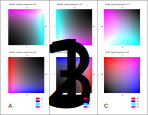
\includegraphics[width=\linewidth]{./images/expressions_fig.png}
\caption{Retinal and tectal gene expression.
%
\textbf{A} Retinal receptor expression. Four receptors are expressed and
displayed here in two dual-colour maps. $r_0$ and $r_1$ are red and
green;$r_2$ and $r_3$ are cyan and magenta. $r_0$ increases as an
exponential function of $x$; $r_1$ increases with an exponential function of
$y$. $r_2$ and $r_3$ have the opposite sense. The expression is modelled with
exponential functions because there is ample evidence that shows that retinal
receptor expressions follow this form.
%
\textbf{B} Retinal ligand expression. May not be included.
%
\textbf{C} Tectal receptor expression. May not be included.
%
\textbf{D} Tectal ligand expression. $l_0$ and $l_1$ are red and green; $l_2$
and $l_3$ are cyan and magenta. These expressions are shown in a linear form,
as there is less evidence to determine whether tectal ligand expression is
exponential, linear or logarithmic in form.
}
\label{f:1}
\end{figure}

\subsection{Signalling}

In this model, the signal transmitted when a ligand binds to a receptor on a
growth cone can lead to one of two effects; the signal may induce the growth
cone to climb the gradient of ligand expression, in which case the interaction
is \emph{attractive} or the cone may descend the gradient of ligand expression
if the interaction is \emph{repulsive}.

Based on a Michaelis-Menten model applied to
receptor-binding, \citet{mortimer_bayesian_2009} give an expression for the
probability of an individual receptor being bound as a function of the ligand
expression, $\gamma$, and the ligand gradient, $\mu$;
\begin{equation}
P(b=1|\gamma,\mu) = \frac{\gamma(1 + \mu r)}{1 + \gamma(1 + \mu r)},
\end{equation}
where $r$ is the distance of the receptor from the centre of a 1D growth
cone. To determine the sampled direction signal (for one dimension), we assume
evenly spaced receptors and sample from a uniform distribution for each
location across the growth cone.

This is where I really want to say ``the only interactions in the model are
via forward (ligand-activates-receptor) and reverse
(receptor-activates-ligand) signalling''. Something like:

Interactions in the model are by receptor-ligand interactions only. Forward
interactions are those in which the ligand activates the receptor, delivering
a signal into the receptor-expressing cell. Reverse signals occur when a
membrane-bound ligand is activated~\citep{wu_role_2019}.

\section{Results}

\section{Discussion}

% Discuss the Hill Equation! https://en.wikipedia.org/wiki/Hill_equation_(biochemistry)
% This relates to the work \cite{naoki_revisiting_2017}

%
% BIBLIOGRAPHY
%
\selectlanguage{English}
\bibliographystyle{apalike}
\bibliography{RetinoTectal}

\end{document}
